\section{Introduction}





\subsection{Fire safety science}





\begin{frame}
\frametitle{Fire safety science}

\begin{itemize}
\item Civilian safety in metro stations
  \begin{itemize}
  \item Smoke spread in case of fire
  \item Egress routes for pedestrians
  \end{itemize}
\end{itemize}

\vfill{}

\begin{itemize}
\item Individual examinations necessary on complex geometries
\item Experiments expensive $\longrightarrow$ Alternative: Computer simulations
\end{itemize}

\begin{minipage}{.49\textwidth}
  \begin{figure}
  \includegraphics[width=\textwidth]{figures/2017_januar_experimente_lukas_28_450px.png}
  \caption{Experiments in metro}
  \end{figure}
\end{minipage}
\hfill{}
\begin{minipage}{.49\textwidth}
  \begin{figure}
  \includegraphics[width=\textwidth]{figures/2017_februar_verbundtreffen_hamburg_002_450px.png}
  \caption{Physical model (scale 1:15)}
  \end{figure}
\end{minipage}
\end{frame}





\begin{frame}
\frametitle{Fire simulation}

\begin{itemize}
\item Lots of software tools available: FDS, FireFOAM, Ansys Fluent, \ldots
\item Flexible: Scenarios may be varied easily
\end{itemize}

\vfill{}

\begin{itemize}
\item \textbf{But:} Large and complex geometries yield lots of workload
\item Simulations require a lot of time
\end{itemize}

\vfill{}

\begin{minipage}[b]{.49\textwidth}
  \begin{figure}
  \includegraphics[width=\textwidth]{figures/deflagration_heptane_500kg_450px.png}
  \caption{Deflagration of Heptane}
  \end{figure}
\end{minipage}
\hfill{}
\begin{minipage}[b]{.49\textwidth}
  \begin{figure}
  \includegraphics[width=\textwidth]{figures/metro_cad_450px.png}
  \caption{CAD model}
  \end{figure}
\end{minipage}
\end{frame}




\subsection{Computation fluid dynamics}





\begin{frame}
\frametitle{Computational fluid dynamics}

\begin{itemize}
\item Smoke spread modeled with incompressible Navier--Stokes equations
  \begin{align*}
  \nabla \cdot \vectorsym{u}
  &= 0
  \\
  \rho_0 \left[ \partial_t \vectorsym{u} + \left( \vectorsym{u} \cdot \nabla \right) \vectorsym{u} \right]
  &= - \nabla p + \nabla \cdot \left( 2 \, \mu \, \tensorsym{\epsilon} \right) +  \vectorsym{f}
  \\
  \rho_0 c_p \left[ \partial_t T + \left( \vectorsym{u} \cdot \nabla \right) T \right]
  &= 2 \, \mu \, \tensorsym{\epsilon} : \nabla \vectorsym{u} + \nabla \cdot \left( \kappa \, \nabla T \right) + q - \vectorsym{u} \cdot \vectorsym{f}
  \end{align*}
\end{itemize}

\vfill{}

\begin{itemize}
\item Solution via numerical methods $\longrightarrow$ Computational fluid dynamics
\item High resolution necessary for \ldots
\begin{itemize}
  \item Large gradients in temperature and velocity
  \item Turbulence
  \item Flow separation
\end{itemize}
\end{itemize}
\end{frame}





\begin{frame}
\frametitle{Motivation for PhD project}

\begin{itemize}
\item Fires stay localized in general, not only during ignition phase
\item Unnecessarily fine grids bind resources that could be used near the fire
\item Demand for effective use of computing power
\end{itemize}

\vfill{}

\begin{block}{Goal}
\begin{itemize}
\item Balance accuracy and workload by adapting resolution
\item Accelerate simulations by exploiting hardware
\end{itemize}
\end{block}

\begin{center}
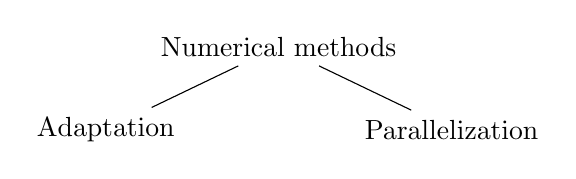
\begin{tikzpicture}[level distance=3em]
\node {Numerical methods} [sibling distance=12.5em]
child { node {Adaptation} }
child { node {Parallelization} };
\end{tikzpicture}
\end{center}
\end{frame}





\begin{frame}
\frametitle{Example: Adaptive mesh refinement}

\begin{itemize}
\item Demonstration of adaptive mesh refinement (\h-adaptive methods) via moving vortex test case as a shape-preserving potential stream.
\end{itemize}

\begin{figure}
\centering
%\movie[externalviewer]{\includegraphics[width=\textwidth]{movies/amrvortex_1pass_teaser.png}}{movies/amrvortex_1pass.avi}
\href{run:movies/amrvortex_1pass.avi?loop&poster}{\includegraphics[width=\textwidth]{movies/amrvortex_1pass_teaser.png}}
\caption{Video of velocity magnitude of moving vortex, overlaid with current mesh}
\end{figure}
\end{frame}





\begin{frame}
\frametitle{Numerical methods}

\begin{minipage}[t]{.3\textwidth}
\begin{center}
\Large{Finite differences}

\vspace{1em}
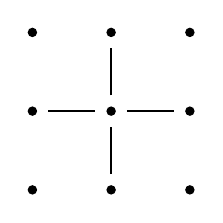
\begin{tikzpicture}
\foreach \x in {0,1,2}
\foreach \y in {0,1,2}
\fill (\x,\y) circle (.06cm);

\draw[thick] (0+0.2,1) -- (1-0.2,1);
\draw[thick] (1+0.2,1) -- (2-0.2,1);
\draw[thick] (1,0+0.2) -- (1,1-0.2);
\draw[thick] (1,1+0.2) -- (1,2-0.2);
\end{tikzpicture}
\end{center}

Difference quotients as differential operators
\end{minipage}
\hfill
\begin{minipage}[t]{.3\textwidth}
\begin{center}
\Large{Finite volumes}

\vspace{1em}
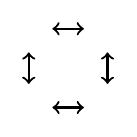
\begin{tikzpicture}
\LagrangeCell{0}{0}{1}{0.06}{1}{{,,,}};
\LagrangeCell{1}{0}{1}{0.06}{1}{{,,,}};
\LagrangeCell{0}{1}{1}{0.06}{1}{{,,,}};
\LagrangeCell{1}{1}{1}{0.06}{1}{{,,,}};

\draw[<->,thick] (0.5,1-0.2) -- (0.5,1+0.2);
\draw[<->,thick] (1.5,1-0.2) -- (1.5,1+0.2);
\draw[<->,thick] (1-0.2,0.5) -- (1+0.2,0.5);
\draw[<->,thick] (1-0.2,1.5) -- (1+0.2,1.5);
\end{tikzpicture}
\end{center}

Balance fluxes on faces between volumes\\[.5em]
Conservation laws
\end{minipage}
\hfill
\begin{minipage}[t]{.3\textwidth}
\begin{center}
\Large{Finite elements}

\vspace{1em}
\begin{tikzpicture}
\LagrangeCell{0}{0}{1}{0.06}{2}{{,,,,,,,,}};
\LagrangeCell{1}{0}{1}{0.06}{2}{{,,,,,,,,}};
\LagrangeCell{0}{1}{1}{0.06}{2}{{,,,,,,,,}};
\LagrangeCell{1}{1}{1}{0.06}{2}{{,,,,,,,,}};
\end{tikzpicture}
\end{center}

Limit function space to piecewise polynomials
\end{minipage}

\vspace{1.5em}

\begin{minipage}[t]{.3\textwidth}
%Structured grids\\[.5em]
\h-adaptive methods
\end{minipage}
\hfill
\begin{minipage}[t]{.3\textwidth}
%Unstructured grids\\[.5em]
\h-adaptive methods
\end{minipage}
\hfill
\begin{minipage}[t]{.3\textwidth}
%Unstructured grids\\[.5em]
\hp-adaptive methods
\end{minipage}
\end{frame}